% 20220087 ICACT 2020 submission code


\documentclass[conference]{IEEEtran}
\IEEEoverridecommandlockouts
% The preceding line is only needed to identify funding in the first footnote. If that is unneeded, please comment it out.
\usepackage{cite}
\usepackage{amsmath,amssymb,amsfonts}
\usepackage{algorithmic}
\usepackage{graphicx}
\usepackage{textcomp}
\usepackage{xcolor}
\def\BibTeX{{\rm B\kern-.05em{\sc i\kern-.025em b}\kern-.08em
    T\kern-.1667em\lower.7ex\hbox{E}\kern-.125emX}}
\begin{document}

% Department of Computer Sciences,
% Division of Science and Technology,
% Graduate School of Technology, Industrial and Social Sciences,
% Tokushima University



\title{Shadowing-Fading-based Intersection Geographic Opportunistic Routing Protocol for Urban VANETs}
\author{
\IEEEauthorblockN{Shuto Takahashi*, Masami Yoshida*, Alberto Gallegos Ramonet**, Taku Noguchi*** }
\\
\IEEEauthorblockA{
\textit{ *Graduate School of Information Science and Enginieering, Ritsumeikan University, } Shiga, Japan \\
\textit{**Department of Computer Sciences,
Division of Science and Technology,} \\
\textit{Graduate School of Technology, Industrial and Social Sciences}
\textit{Tokushima University,} Tokushima, Japan \\
\textit{***College of Information Science and Engineering, Ritsumeikan University,} Shiga, Japan \\
}

\IEEEauthorblockA{ 
\textbf{*\{is0361er, is0195hr\}@ed.ritsumei.ac.jp}
\textbf{**alramonet@is.tokushima-u.ac.jp }
\textbf{***noguchi@is.ritsumei.ac.jp}
}

% \IEEEauthorblockA{\textit{***College of Information Science and Engineering, Ritsumeikan University} \\
% Shiga, Japan \\  }

}





\maketitle

\begin{abstract}

In vehicular ad-hoc networks (VANETs), the presence of obstacles such as buildings and trees cause shadowing and fading, which interfere with the propagation of radio waves. Despite this, most of the existing opportunistic routing protocols do not consider shadowing in  their simulations, which may lead to an overestimation of VANET performance. 
To solve this problem, our proposed routing protocol can minimize the effect of shadowing by actively selecting street intersection nodes as relay nodes. 
% In this study, we investigated the effect of shadowing on an existing routing protocol, link state aware geographic opportunistic (LSGO) routing, using a shadowing obstacle model implemented in ns-3.
In this study, we propose a shadowing-fading -based intersection geographic opportunistic routing protocol (SIGO). 
SIGO determines the priority of a relay node by considering the distance between the relay node and the destination node, the link quality between these nodes, and a street intersection relay index (IRI) in which the best relay node is selected according to the influence of shadowing.
Through simulations, we demonstrated the effectiveness of SIGO' communication performance in terms of an improvement in the packet delivery ratio and the decrease in end-to-end delay.

\end{abstract}

\begin{IEEEkeywords}
VANET, Routing Protocols, Opportunistic Routing Protocols, Shadowing
\end{IEEEkeywords}

\section{Introduction}
Intelligent transportation systems (ITS) \cite{1} have been actively pursued to improve the safety and convenience of driving and  reduce the environmental impact. 
Vehicle ad-hoc networks (VANETs), made possible by inter-vehicle communication, are essential for various applications in ITS.
In VANETs,  ad-hoc communication is achieved between vehicles equipped with wireless communication devices, enabling the construction of flexible networks. 
When VANETs are deployed in  urban environments, fast node mobility, heterogeneity, and the presence of buildings must be considered in the performance evaluation. A wide variety of routing protocols have been proposed to meet various requirements \cite{2}.
The existing routing protocols in VANETs can be classified into two categories: topology-based routing protocols and geographic routing protocols. Topology-based routing protocols \cite{3,4,5} use network link information to forward packets. 
Additionally, these routing protocols are not suitable for VANETs because they cannot support fast node movements. In contrast, geographic routing protocols \cite{6, 7, 8 ,9} can forward packets based on the location information of neighboring nodes and destination node location. 
In this type of routing protocol, nodes do not need to maintain established routes, as in conventional mobile ad-hoc network routing protocols. 
Therefore, the geographic routing protocol can cope with topology changes with a small number of packets.
Greedy forwarding is one of the most widely used packet forwarding methods for geographic routing protocols.
However, in an actual urban environment, the drop rate of packets may increase because of shadowing and degradation of signal strength over a distance. This increases the possibility of packet retransmission, resulting in increased overhead and end-to-end delay. 

Opportunistic routing protocols have attracted attention in contrast to these methods \cite{16}. 
The main difference between opportunistic routing protocols and conventional routing schemes is that opportunistic routing protocols do not use a fixed route, but allow nodes that receive packets to decide whether to forward them. 
This can increase the chance of receiving packets and, consequently, achieve better performance compared with conventional routing schemes.
However, most of the existing originally opportunistic routing protocols  are not designed for urban environments; therefore, their performance evaluation does not take into account the effect of \textit{shadowing fading} caused by buildings, which may result in an overestimation of the communication performance. 
In fact, it has been demonstrated that buildings attenuate the radio wave of 802.11p channels, and that data transmission is limited along the road\cite{17}. 

In this study, we evaluate the link state aware geographic opportunistic (LSGO)
routing protocol for VANETs \cite{18}, using an obstacle shadowing model \cite{20}. 
Our evaluations tested the LSGO under the obstacle shadowing model \cite{20} using the ns-3 network simulator \cite{19}. 
We also tested the protocol performance when shadowing is not considered.
Additionally, we proposed a new routing protocol called the shadowing-fading-based intersection geographic opportunistic (SIGO) routing protocol to improve the communication performance in shadowing environments.
In the SIGO protocol, we consider the distance to the destination node and the expected transmission probability. Furthermore, SIGO considers whether a node is close to a street intersection node  when selecting the relay nodes.
Our evaluations demonstrated the effectiveness of the proposed method in a simulation environment. 
The rest of this paper is organized as follows:
% Section \ref{relatedSection} describes the existing opportunistic routing protocols and shadowing. 
% Section \ref{LSGO} describes LSGO. 
Section \ref{relatedSection} describes the existing opportunistic routing protocols.
Section \ref{SIGO} describes the proposed method (SIGO), and Section \ref{evaluation} presents the performance evaluation and effectiveness of the proposed method. Finally, Section \ref{conclusion} summarizes our conclusions and discusses future work.





\section{RELATED WORK} %----------------------
\label{relatedSection}

% \subsection{Opportunistic Routing Protocols Background}

Compared with conventional geographic routing protocols \cite{6}, opportunistic routing protocols improve communication performance by increasing the number of opportunities for relay nodes to receive packets. Figure \ref{fig:Basic} shows the basic model of the opportunistic routing protocols.

\begin{figure}[!ht]
\centering
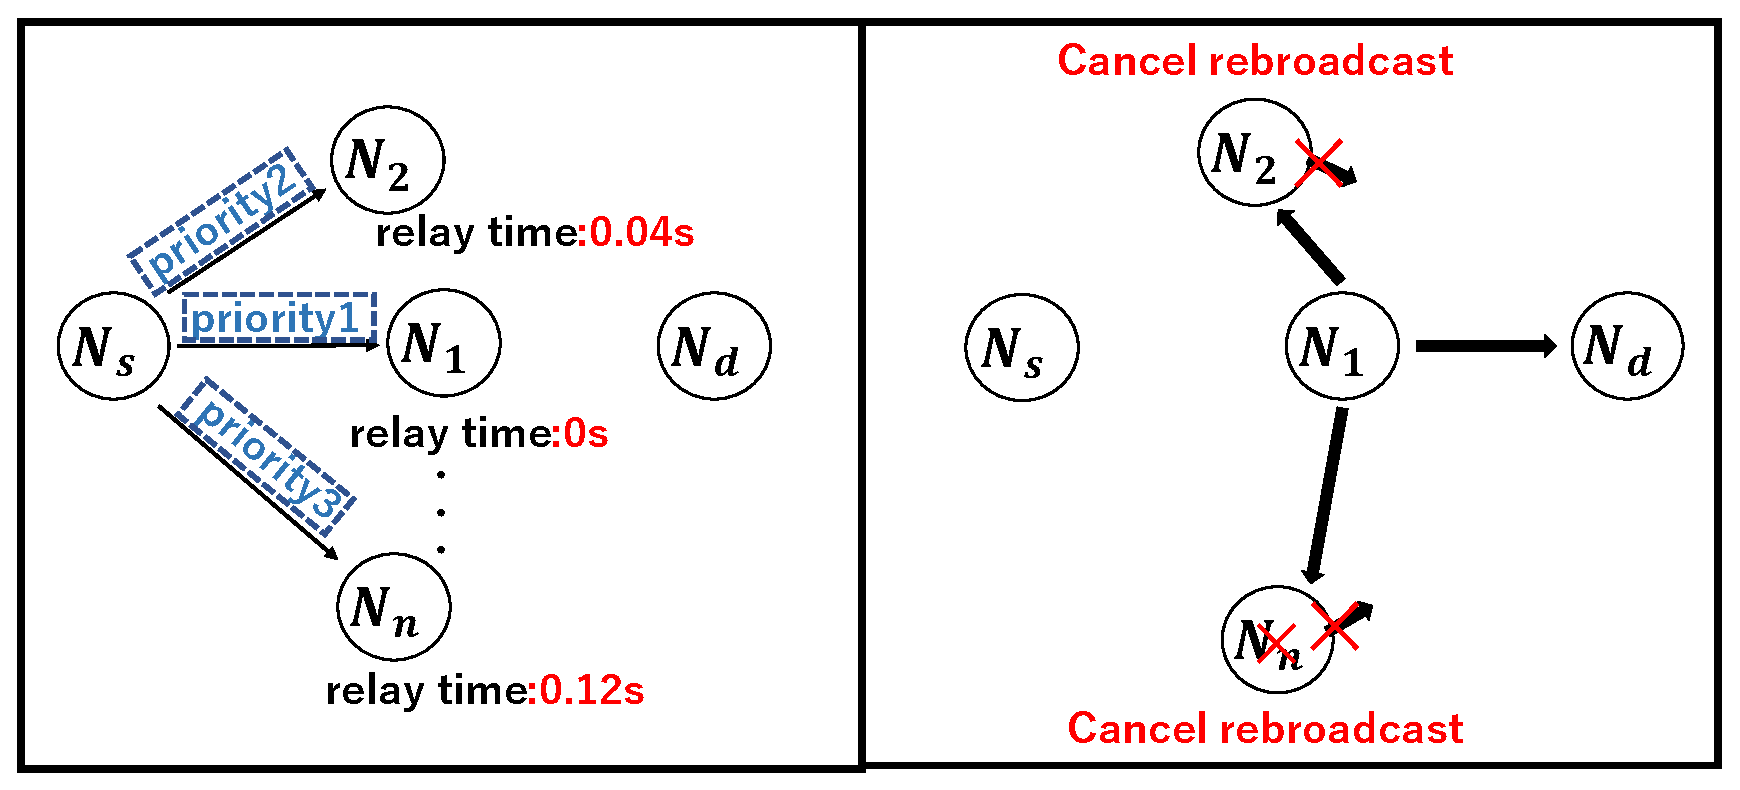
\includegraphics[width=80mm]{figures/basic-opportunity2.eps}
\caption{The basic model of opportunistic routing protocols}
\label{fig:Basic}
\end{figure}


Node $N_{s}$ selects a candidate node for relaying and determines the priority from $N_{1}$ to $N_{n}$. Subsequently, $N_{s}$ writes the priorities of $N_{1}$ to $N_{n}$ in the packet and broadcasts it. 
In each packet of the figure, the priority of the relay node is described for the sake of clarity, but the actual packet is broadcast, and thus, the contents of the packet are identical. 
The nodes that receive the packet set a relay timer according to their own priority.
The higher the priority, the smaller the relay timer is set.
The nodes that time out will rebroadcast packets.
In addition, each relay node cancels its rebroadcast when it overhears the transmission of the packet from a node with a higher priority than itself.
before its timer expires, thereby preventing the increase of redundant packets.
These results show that in opportunistic routing protocols, the priority-determination algorithm directly affects  the communication performance.


Opportunistic multi-hop routing for wireless
networks (ExOR) \cite{16} have been proposed as typical opportunistic routing protocols. It determines the priority of relay nodes by using the original expected transmission cost (ETX) \cite{21}. However, this newly devised method for calculating the ETX value has a problem in that it does not take into account the random and fast mobility nature of nodes, which is a characteristic of VANET nodes.\par


Therefore, LSGO devised a new ETX value suitable for VANETs. In LSGO, the ETX value is used as a metric to determine the priority, which improves the packet delivery ratio (PDR) and reduces the end-to-end delay.
In the collision-aware opportunistic routing protocol (SCAOR) \cite{22}, node density is added as a metric in the priority determination to prevent packet collisions that degrade network performance. 
As a result, the performance is improved compared with LSGO and EXOR in a highway deployment environment. 
In the hybrid opportunistic and position-based routing protocol (OPBR) for VANETs
\cite{23}, to solve the problem of delay increase when the packet does not reach the relay node, OPBR infers the link breakage of the neighboring node from the location information gathered from the neighboring nodes.


However, a  common issue in all of these protocols is that they do not consider shadowing.
This problem causes these protocols to overestimate communication performance. 
% In Section \ref{LSGO}, we examine the impact of shadowing on the communication performance of LSGO using simulations. 


% \subsection{Shadowing fading}
% When designing routing protocols for VANETs, many studies consider the fast mobility of nodes, deviating node density, and link instability. 
% However, VANETs are often assumed to be deployed in urban environments; therefore, it is essential to design routing protocols that consider the effects of shadowing. 
% The 802.11p channel commonly used in VANETs is shown to have a lower packet delivery ratio (PDR) in real-world measurements because of the influence of buildings \cite{17}.
% As shown in Figure \ref{fig:Gray-Zone}, the 802.11p channel commonly used in VANETs has a lower packet delivery ratio (PDR) in real-world measurements in the gray zone \cite{17} located on the side of the streets because of the influence of buildings.

% \begin{figure}[!ht]
% \centering
% 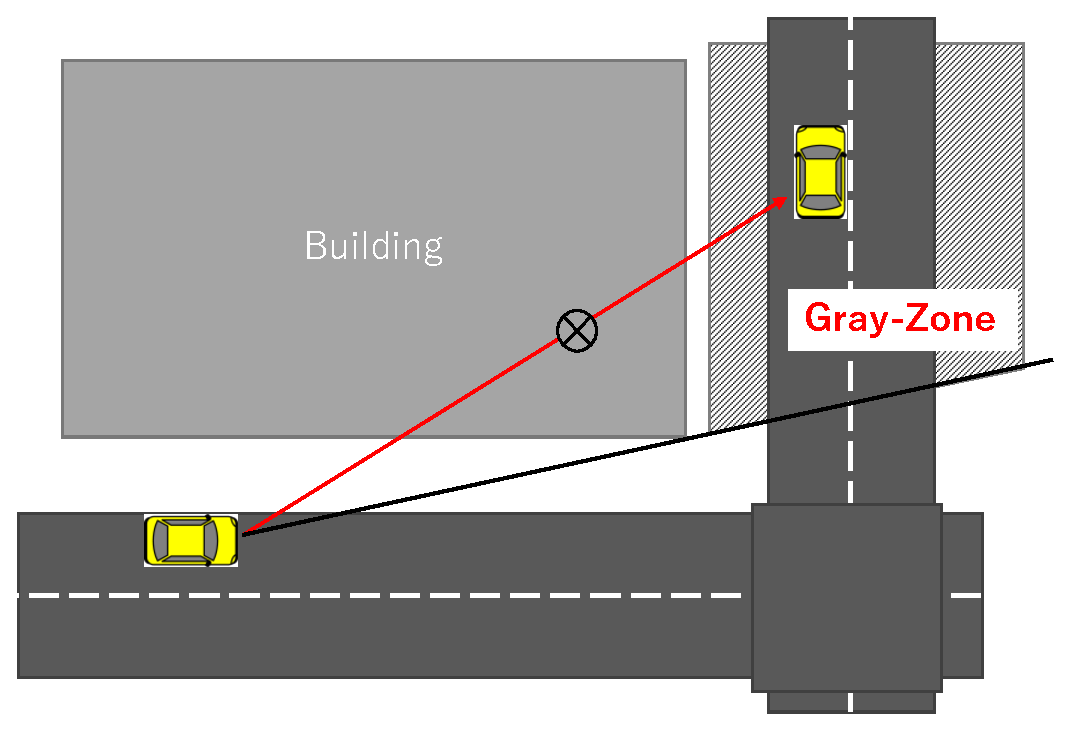
\includegraphics[width=90mm]{figures/Gray-Zone.eps}
% \caption{The gray-zone in an intersection }
% \label{fig:Gray-Zone}
% \end{figure}



% Intersection-based selection routing protocols \cite{24,25,26}  are effective for shadowing problems.
% The forwarding strategy of these protocols can be divided into three steps. The first is intersection selection, the second is road selection at the intersection, and the third is forwarding on the selected road. 
% In these intersection-based routing approaches, the impact of shadowing fading can be minimized because packets are forwarded along the road.
% However, when packets are forwarded linearly, as shown in Figure \ref{fig:intersection_routing}, extra hop relays are introduced for each intersection in an intersection-based selection routing. These extra hop relays result in unnecessary relays and increase the overall delay.




% \begin{figure}[!ht]
% \centering
% 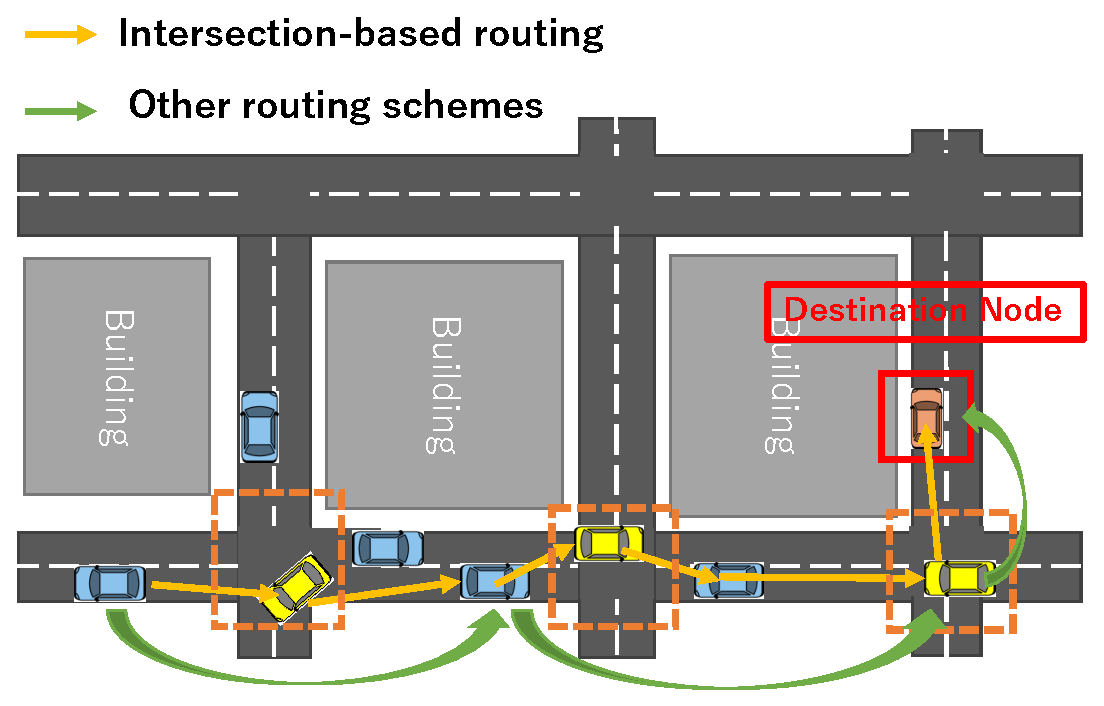
\includegraphics[width=85mm]{figures/intersection_routing.eps}
% \caption{Cases where intersection-based routing is inefficient}
% \label{fig:intersection_routing}
% \end{figure}

% \section{LSGO}
% \label{LSGO}

% In LSGO, each node periodically broadcasts a $hello$ packet consisting of the node ID and its current position coordinates (x,y). 
% The node that receives the data packet  selects some relay candidate nodes based on the  information collected from the hello packets  of neighboring nodes to deliver the data packet to the destination node. 
% Then, it assigns a priority to the selected candidate nodes and rebroadcasts the received packet. 
% The transmitting node  determines the priority of the candidate nodes according to  the algorithm described below. 
% In LSGO, the priority of relay candidate nodes is determined based on two metrics: link quality and distance to the destination. 
% Each node that receives the data packet checks whether it contains its own ID and discards the packet if it does not.
% The node checks its own priority and rebroadcasts the packet according to the priority-scheduling algorithm if the ID  is valid.


% \subsection{Link quality estimation}

%   In LSGO, each node broadcasts a hello packet periodically, and hello packets are used to measure the expected transmission probability of neighboring nodes. The transmitted hello packets consist of the node ID and node position coordinates (X,Y). To calculate the ETX of a link, each node should record $t_{0}$, which is the time when the first hello packet is received and the number of packets it receives from the neighbor during the last $w$ seconds. Then, according to the interval between $t_{0}$ and the current time $t$ and window $w$, the expected probability of successful transmission $r(t)$ is calculated by Equation (\ref{trans-prediction})

% \begin{equation}
% \label{trans-prediction}
% r(t) =\begin{cases}count(t, t_{0}), & 0 < t - t_{0} < 1,  \\ \frac{count(t,t_{0})}{(t-t_{0}) / \tau}, & 1 \leq t - t_{0} \leq w\\
% \frac{count(t - w,t)}{w / \tau}, &  t - t_{0} \geq w\\
% \end{cases}
% \end{equation}

% The denominator is the number of hello packets that should have been received during the window, and $\tau$ represents the broadcast interval of the hello packets. $count(t,t_{0})$ is the number of hello packets received during $t$-$t_{0}$.  
% As can be seen from the equation, there are three situations in terms of the difference between $t$-$t_{0}$ and window time $w$. (1) 0 < $t$-$t_{0}$ < 1, where the packet delivery ratio is the number of hello packets received from $t_{0}$ to $t$. (2) 1 $\leq$ $t$-$t_{0}$ < $w$, where the packet delivery ratio is the number of hello packets received from $t_{0}$ to $t$ divided by the length of this period. (3) $t$ - $t_{0}$ $\geq$ $w$, which is the same as the calculation in the ETX metric.

% In LSGO, the asymmetry of the link is not considered, and only the expected probability of one-way transmission is used to calculate the link ETX. 
% Assuming that the expected probability of a one-way transmission is $r(t)$, then the link ETX is calculated using Equation (\ref{equ-intersection}).
 
%  \begin{equation}
%  \label{equ-intersection}
%  ETX = \frac{1}{  {r(t)}^{2}   } 
%  \end{equation}



% \subsection{Priority scheduling algorithm}
% LSGO uses a timer-based priority-scheduling algorithm, in which the highest priority node sends the packet first. If other candidate nodes hear a higher-priority node sending a packet, they would not process the packet; if the timer expires and a higher-priority node is not transmitting, they would begin to send the packet. LSGO calculates the priority of node $i$ according to Equation (\ref{LSGO-priority}) below.

% \begin{equation}
% \label{LSGO-priority}
% \frac{D_{sd} - D_{id}}{ETX_{i}^{2}} ,   D_{id} < D_{sd}
% \end{equation}

% where $D_{sd}$ is the distance from the transmitting node to the destination node, and $D_{id}$ is the distance from candidate node $i$ to the destination node. In addition, \mbox{$D_{sd}$ - $D_{id}$ }is a distance metric. If the condition $D_{id}$ < $D_{sd}$ is not satisfied, the node is excluded from the relay candidate nodes without calculating its priority. The larger the value calculated in Equation (\ref{LSGO-priority}), the higher the priority of node $i$. 

% \subsection{Influence of shadowing}
% \label{shadowing_evaluation}
% In this section, we explain the difference between the communication performance of LSGO with and without radio attenuation caused by shadowing. 


% \subsubsection{Simulation Settings} 
% The simulation parameters are shown in Table \ref{tab:parameter}. 
% The simulation topology scenario was created using SUMO \cite{27}, as shown in Figure \ref{fig:scenario}. 

% \begin{figure}[!ht]
% \centering
% 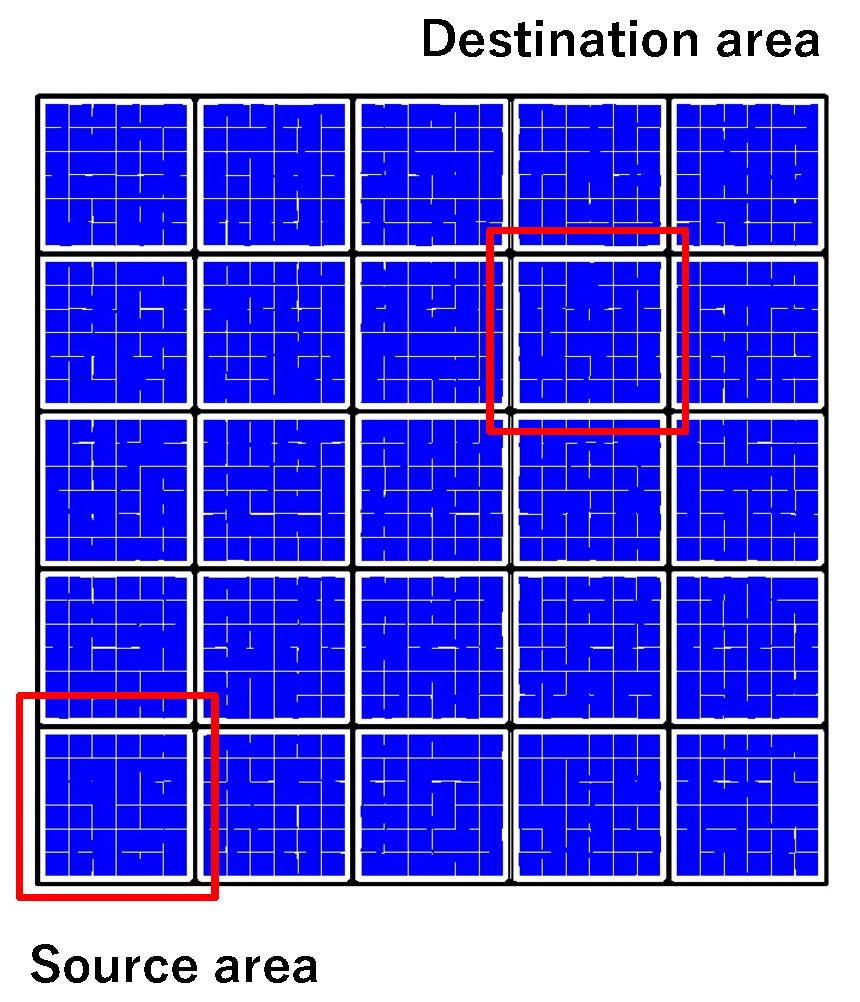
\includegraphics[width=80mm]{figures/scenario.eps}
% \caption{simulation scenario }
% \label{fig:scenario}
% \end{figure}


% Ten source node and destination node pairs were randomly selected from the source and destination areas in Figure \ref{fig:scenario}.
%  Traffic signals were placed at each intersection, and buildings were placed as shown in the blue area of Figure \ref{fig:scenario}. 
% The obstacle shadowing model \cite{20} was used as the radio wave propagation model. The obstacle shadowing propagation loss $L_{s,o}$ is calculated based on the loss for each wall and the distance (m) through the building, as shown in Equation (\ref{shadowing}).

% \begin{equation}
% \label{shadowing}
% L_{s,o} = \alpha n  + \beta d_0
% \end{equation}

% where $\alpha$ is the attenuation per wall (dB), and $n$ is the number of walls penetrated. 
% $\beta$ is the attenuation per meter (dB), and $d_0$ is the distance traveled through obstacles (m). 
% In this simulation experiment, $\alpha$= 10 dB and $\beta$= 0.4 $ dB $ were used in our evaluations. 
% Although an optimized algorithm to select the number of relay candidate nodes was proposed in LSGO, the performance of this algorithm was poor when shadowing propagation loss was used. 
% This algorithm is constructed using the expected transmission probability, r(t). Because the expected transmission probability is calculated from a hello packet, the packet arrives at a higher probability than the transmission probability of the data packet with a larger data size. It is assumed that this is the reason for the performance degradation of the algorithm. 



% \begin{table}[!ht]
% \begin{center}
% \caption{Simulation parameter}
% \label{tab:parameter}
% \begin{tabular}{|l|l|lll}
% \cline{1-2}
% Simulator    & NS-3 (v3.30) &  &  &  \\ \cline{1-2}
% Simulation area    & 1000m × 1000m   &  &  &  \\ \cline{1-2}
% Mobility model     & Random mobility &  &  &  \\ \cline{1-2}
% Transmission range & 250m            &  &  &  \\ \cline{1-2}
% Number of vehicles & 200, 300, 400      &  &  &  \\ \cline{1-2}
% Radio propagation model    & obstacle shadowing model\cite{20}&  &  &  \\ \cline{1-2}
% MAC Layer     & 802.11p &  &  &  \\ \cline{1-2}
% Packet Size & 512 byte       &  &  &  \\ \cline{1-2}
% Simulation Time & 30 s      &  &  &  \\ \cline{1-2}
% hello interval & 1 s      &  &  &  \\ \cline{1-2}
% Window size w  & 10 s      &  &  &  \\ \cline{1-2}
% Number of relay candidate nodes  & 5       &  &  \\ \cline{1-2}
% shadowing parameter $\alpha$  & 10db      &  &  &  \\ \cline{1-2}
% shadowing parameter $\beta$    & 0.4db &  &  \\ \cline{1-2}
% \end{tabular}
% \end{center}
% \end{table}


% \subsubsection{Assessing the influence of shadowing}
% The attenuation impact caused by the buildings on the communication performance of LSGO was evaluated in three evaluation categories: packet delivery ratio, end-to-end delay, and overhead.  

% Figure \ref{fig:LSGO-PDR} shows the packet delivery ratio of the network simulator with and without using the obstacle shadowing loss propagation. 
% The packet delivery ratio is the ratio of the total number of packets received by the destination node to the total number of packets sent by the source node.
% In Fig \ref{fig:LSGO-PDR}, when shadowing is considered in the simulation, the packet delivery ratio decreases for all nodes. This is presumably due to the decrease in the number of candidate nodes for relaying owing to the radio attenuation caused by shadowing.

% \begin{figure}[!ht]
% \centering
% 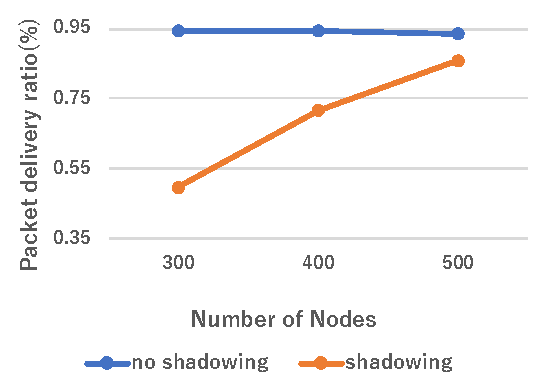
\includegraphics[width=80mm]{figures/LSGO_PDR.eps}
% \caption{Impact of shadowing: PDR }
% \label{fig:LSGO-PDR}
% \end{figure}


% Figure \ref{fig:LSGO-delay} shows the end-to-end delay (s) of the network simulator with and without shadowing effects. The end-to-end delay is defined as the average time between the transmission of a packet by the source node and its successful reception by the destination node.
% In Figure \ref{fig:LSGO-delay}, when shadowing is considered in the simulation, the end-to-end delay increases for all nodes. This is because the attenuation caused by shadowing makes it difficult for packets to pass through the buildings to reach the destination node, making it difficult to form a linear path between the source and destination nodes.

% \begin{figure}[!ht]
% \centering
% 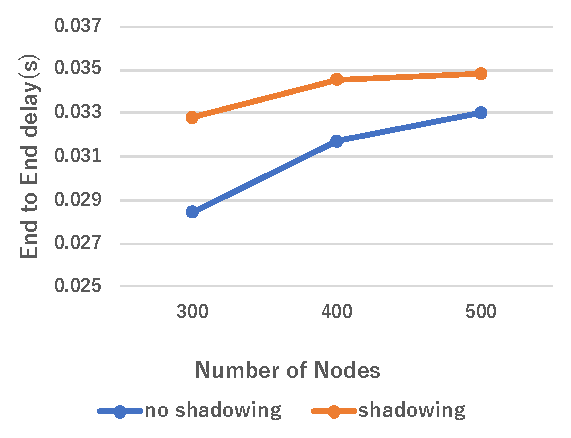
\includegraphics[width=80mm]{figures/LSGO_delay.eps}
% \caption{Impact of shadowing: delay}
% \label{fig:LSGO-delay}
% \end{figure}

% Figure \ref{fig:LSGO-overhead} shows the overhead of LSGO with and without the shadowing effect. 
% The overhead is the total number of data packets transmitted by all nodes in the entire network divided by the total number of data packets successfully received by the destination nodes.
% In \mbox{Figure \ref{fig:LSGO-overhead}}, the overhead increases for all nodes when shadowing is considered in the simulation.
% The algorithm works to cancel rebroadcast between relay candidate nodes according to their priority in opportunistic routing protocols.
% However, because of the shadowing effect, the possibility of not receiving the rebroadcast packet from high-priority nodes increases, and as a result, the overhead is assumed to have increased. 
 

% \begin{figure}[!ht]
% \centering
% 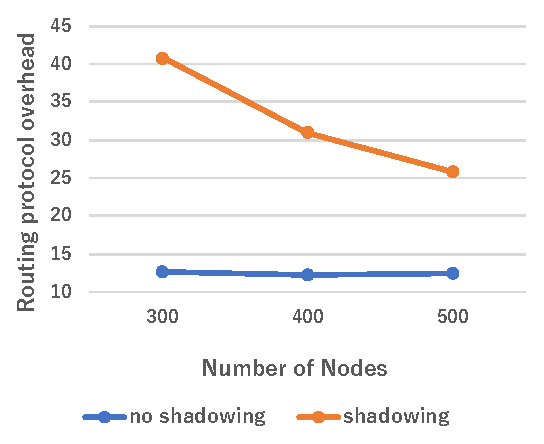
\includegraphics[width=80mm]{figures/LSGO_overhead.eps}
% \caption{Impact of shadowing: overhead}
% \label{fig:LSGO-overhead}
% \end{figure}

% \subsection{Problems with LSGO}

% In this section, we discuss the problems of the LSGO relay strategy.  
% In the forwarding strategy of LSGO, a node that is closer to the destination node and has better link quality is more likely to be selected as a forwarding node. 
% An example of this simulation is shown in Figure \ref{fig:LSGO-route} (a). 
% Consider the situation where node B is selected as the forwarding node, as shown in this Figure. 
% In this case, the following relay nodes after node B (selected from nodes closer to the destination node than node B) are only nodes C and D with poor link quality due to shadowing.  
% We call this problem the $local$ $shadowing$ $problem$. 
% Occasionally, it is possible  that the links with nodes C and D do not exist entirely  because of  shadowing. 
% In these cases, the problem is that there is no longer a node close to the destination other than  node B. 
% This has long been a problem in  location-based routing protocols and is called the local optimum problem. 
% From the above, we can see that the LSGO forwarding strategy is likely to fall into the local optimum problem and the local shadowing problem. This problem may be solved by selecting a street intersection node, such as node A, as a relay node, as shown in \mbox{Figure \ref{fig:LSGO-route} (b)}. 




% \begin{figure}[!ht]
% \centering
% 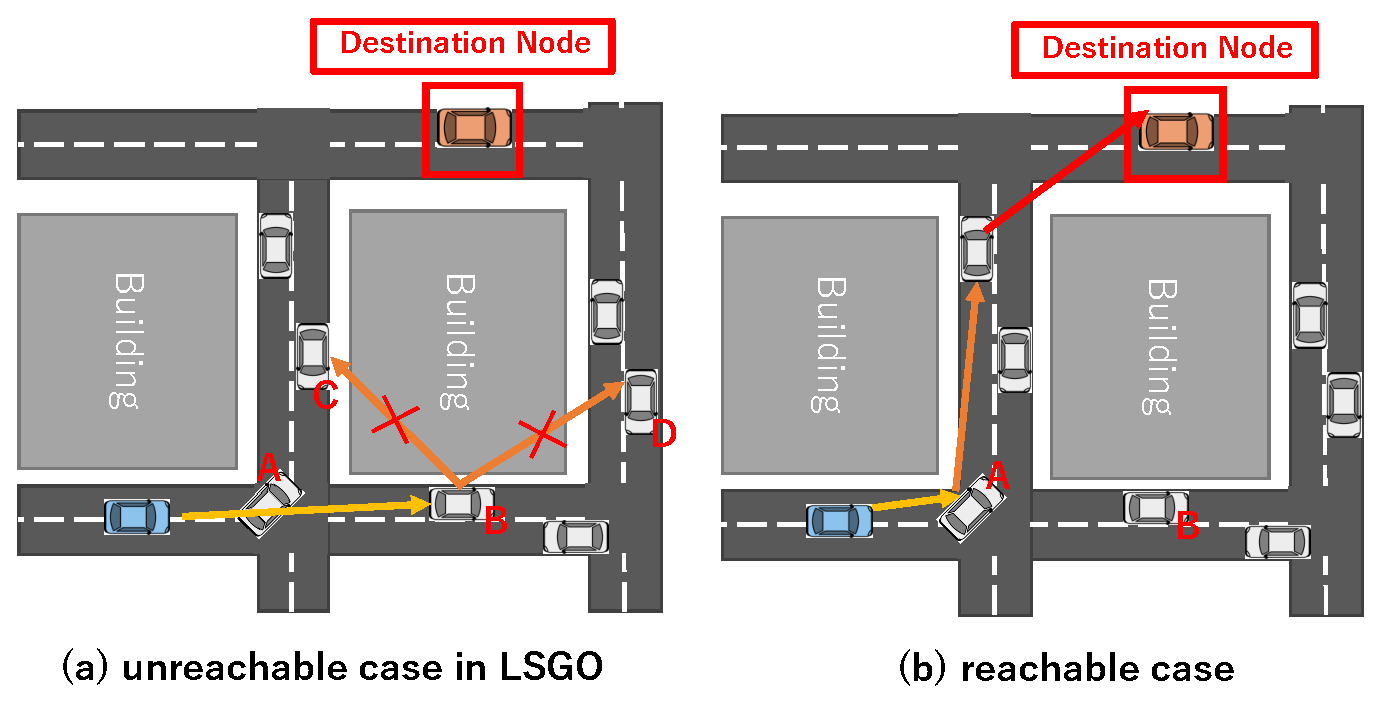
\includegraphics[width=90mm]{figures/efficient_route.eps}
% \caption{Forwarding node selection problem}
% \label{fig:LSGO-route}
% \end{figure}
% --------------------------------------------------------------------


\section{The proposed scheme}
\label{SIGO}
In this study, we propose a new opportunistic routing protocol named SIGO that considers street intersections. 
In SIGO, the priority of relay nodes is determined based on three metrics: distance to destination, link quality, and a street intersection relay index ($IRI$), which is used to give priority to nodes in the intersection.
The first two metrics, distance to destination and link quality, were calculated in the same way as in LSGO. 
In SIGO, as in LSGO, each node periodically broadcasts hello packets. To deliver the packets to the destination node, the transmitting node selects several relay candidate nodes among the neighboring nodes based on the information in the hello packets and broadcasts the data packets containing the priority information of each relay candidate node.

The transmitting node determines the priority of the relay candidate nodes according to the algorithm described 
below. Each node that receives a data packet checks whether it contains its ID and discards the packet if it does not. If the ID is included, the node checks its priority and decides whether to rebroadcast the packet according to the \textit{priority scheduling algorithm} described in \mbox{Section \ref{priority}}.

\subsection{Basic assumption and terminology}
In SIGO, we have made the following definition and assumptions.
\begin{itemize}
\item A \textit{road segment} is defined as a part of the road which connects two unique street intersections.
\item All nodes are equipped with GPS and have access to digital maps.
\item Each node can identify the road segments and the street intersections where its neighbor nodes exist since it
periodically receives hello packets from its neighbor nodes.
\end{itemize}


\subsection{SIGO hello and data packet format}
In SIGO, each node periodically broadcasts a hello packet to keep track of its neighbors' link quality and location. The hello packet contains the following information. 

\begin{itemize}
\item $ID$: The identifier of the node that generates the hello packet.
\item $X$: The $x$-coordinate value.
\item $Y$: The $y$-coordinate value.
% \item $v$: The speed.
% \item $a$: The acceleration.
% \item $\theta$: The direction.
\end{itemize}
% The information of  $v$, $a$, and $\theta$ is used in the \textit{neighbor status prediction} algorithm described in subsection \ref{neighbor_status}.

% \begin{figure}[!ht]
% \centering
% 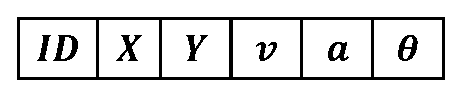
\includegraphics[width=70mm]{figures/Hellopacket_format.eps}
% \caption{The format of hello packet}
% \label{fig:hellopacket}
% \end{figure}

% The structure of the data packet is shown in Figure \ref{fig:datapacket}.
The structure of the data packet is shown below. 
It is assumed that some location information service is used to obtain the location information of the destination node, which is beyond the scope of this study. 
Because SIGO does not use control packets, the priority information assigned to each relay candidate node is included in the data packet.

\begin{itemize}
\item $SourceId$: The source node ID.
\item $DstId$: The destination node ID.
\item $Dst_x Pos$: The $x$-coordinates of the destination node.
\item $Dst_y Pos$: The $y$-coordinates of the destination node.
\item $Id_i$: The relay candidate node ID with priority $i$. $i$ = 1, 2, 3, ...(highest to lowest priority) 
\item $Data$: The data payload.
\end{itemize}

% \begin{figure}[!ht]
% \centering
% 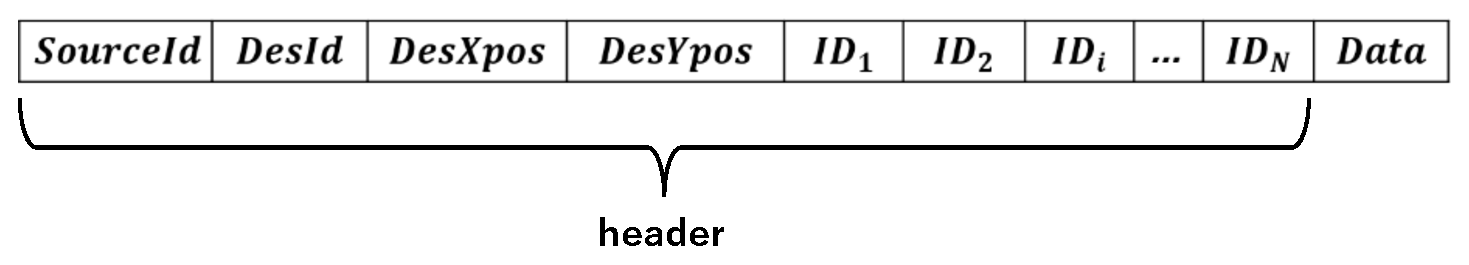
\includegraphics[width=80mm]{figures/data_packet_format.eps}
% \caption{The format of data packet}
% \label{fig:datapacket}
% \end{figure}

\subsection{Link quality estimation}

  In SIGO, each node broadcasts a hello packet periodically, and hello packets are used to measure the expected transmission probability of neighboring nodes. The transmitted hello packets consist of the node ID and node position coordinates (X,Y). To calculate the ETX of a link, each node should record $t_{0}$, which is the time when the first hello packet is received and the number of packets it receives from the neighbor during the last $w$ seconds. Then, according to the interval between $t_{0}$ and the current time $t$ and window $w$, the expected probability of successful transmission $r(t)$ is calculated by Equation (\ref{trans-prediction})

\begin{equation}
\label{trans-prediction}
r(t) =\begin{cases}count(t, t_{0}), & 0 < t - t_{0} < 1,  \\ \frac{count(t,t_{0})}{(t-t_{0}) / \tau}, & 1 \leq t - t_{0} \leq w\\
\frac{count(t - w,t)}{w / \tau}, &  t - t_{0} \geq w\\
\end{cases}
\end{equation}

The denominator is the number of hello packets that should have been received during the window, and $\tau$ represents the broadcast interval of the hello packets. $count(t,t_{0})$ is the number of hello packets received during $t$-$t_{0}$.  
As can be seen from the equation, there are three situations in terms of the difference between $t$-$t_{0}$ and window time $w$. (1) 0 < $t$-$t_{0}$ < 1, where the packet delivery ratio is the number of hello packets received from $t_{0}$ to $t$. (2) 1 $\leq$ $t$-$t_{0}$ < $w$, where the packet delivery ratio is the number of hello packets received from $t_{0}$ to $t$ divided by the length of this period. (3) $t$ - $t_{0}$ $\geq$ $w$, which is the same as the calculation in the ETX metric.

In LSGO, the asymmetry of the link is not considered, and only the expected probability of one-way transmission is used to calculate the link ETX. 
Assuming that the expected probability of a one-way transmission is $r(t)$, then the link ETX is calculated using Equation (\ref{equ-intersection}).
 
 \begin{equation}
 \label{equ-intersection}
 ETX = \frac{1}{  {r(t)}^{2}   } 
 \end{equation}


\subsection{Intersection Relay Index (IRI)}

In SIGO, node $i$ that receives the data packet or the  source node that generates the data packet calculates the 
$IRI$ (intersection relay index) when the following two conditions are satisfied:
\begin{itemize}
\item A street intersection node is closer to the destination node than the source node or the node $i$.
\item There is a street intersection node on an intersection adjacent to the road where the source node and node $i$ exist.
\end{itemize}

The following procedures calculate $IRI$, which gives priority to  the street intersection node.

\textbf{Step1: Selection of the closest road segment.}
To calculate $IRI$, the transmitting node (relay node or the source node) selects one of the road segments closest to the destination node among the road segments where relay candidate nodes exist.
The center coordinate of each road segment was used to calculate the distance between the destination node and road segment. An example is shown in Figure \ref{fig:closest_road}.
The blue vehicle is the transmitting node, the yellow vehicles are the relay candidate nodes, the red vehicle is the destination node, and the green points are the center coordinates of each road segment. In this example, the road segment closest to the destination node is  enclosed by the dashed blue line in the figure.

\begin{figure}[!ht]
\centering
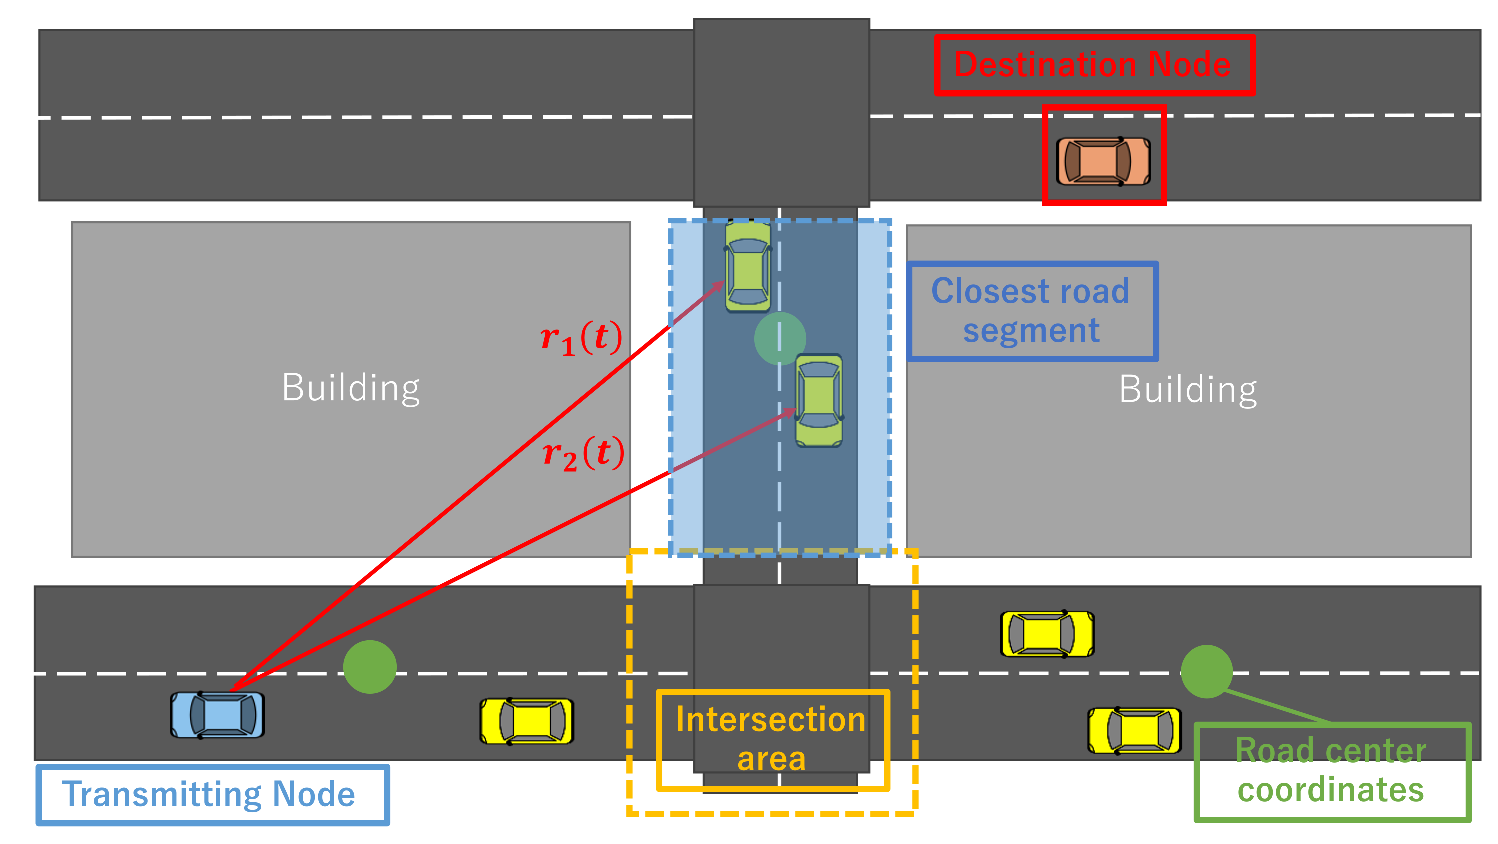
\includegraphics[width=80mm]{figures/closest_road.eps}
\caption{The closest road segment}
\label{fig:closest_road}
\end{figure}


\textbf{Step 2: Calculation of the transmission probability in a selected road segment.}
In this step, the transmitting node calculates the packet reachability probability $R_p$ such that a packet reaches at least one relay candidate node located in the closest road segment calculated in Step 1, using Equation \ref{Rp}.

\begin{equation}
\label{Rp}
R_p = 1 - \prod_{p=1}^N (1 - r_{p}(t))
\end{equation}

where $r_p(t)$ is the expected transmission probability of the relay candidate node $p$ (1 $\leq$  $p$ $\leq$ $N$) in the road segment closest to the destination node. 
$N$ represents the number of candidate nodes in the road segment closest to the destination node. 
The expected transmission probability was calculated using the same equation as in Equation \ref{trans-prediction}.




\textbf{Step3: Calculation of $IRI$.}
Using the $R_p$ calculated in Step 2, the street intersection relay  index $IRI_i$ of neighbor intersection node $i$ is calculated using Equation \ref{IRI}.

\begin{equation}
\label{IRI}
IRI_i = \alpha\frac{90\left(\frac{\theta_I}{90}\right)^\frac{1}{{\gamma}}}{R_p}
\end{equation}
where $\theta_i$ is the angle between the lines connecting the transmitting node to the destination node and  connecting the transmitting node and the intersection node $i$ , as shown in Figure \ref{fig:intersection_angle}.
The higher $\theta_i$  and the lower  $R_p$, the higher the $IRI_i$.
$\alpha$ ($\alpha$ > 0) is a weighting factor of $IRI_i$.
As $IRI_i$ increases, the transmitting node selects the intersection node as a relay node with a higher probability. 
The proposed scheme prioritizes the intersection node as the relay node when $R_p$ is small. 
If $\theta_i$ (|$\theta_i$| <= 90) is large, the communication between the sending node and the candidate relay node that is not an intersection node is more likely to be adversely affected by the shadowing of the building. In other words, when $\theta_i$ is large, an intersection node should be selected as a relay node. Therefore, $IRI_i$ is used for priority calculation in the proposed scheme only when the angle $\theta_i$ is greater than 45 degrees.
% where $\theta_I$ is the angle between the lines connecting the transmitting node to the destination node and  connecting the transmitting node and the intersection node $i$ (Figure \ref{fig:intersection_angle}).
% The higher $\theta_I$  and the lower  $R_p$, the higher the $IRI_i$.
% As $IRI_i$ increases, the transmitting node selects the intersection node as a relay node with a higher probability. 
% The proposed scheme prioritizes the intersection node as the relay node when $R_p$ is small. The node in the selected road segment can receive the packet highly probability by the intersection node's relaying.
% The detailed operation of relay node selection is described in \mbox{Section \ref{priority}}.
% We also add a gamma correction to prevent the intersection node from being given too much priority when $\theta_I$ is small.
% where $\gamma$ is the gamma correction value.


\begin{figure}[!ht]
\centering
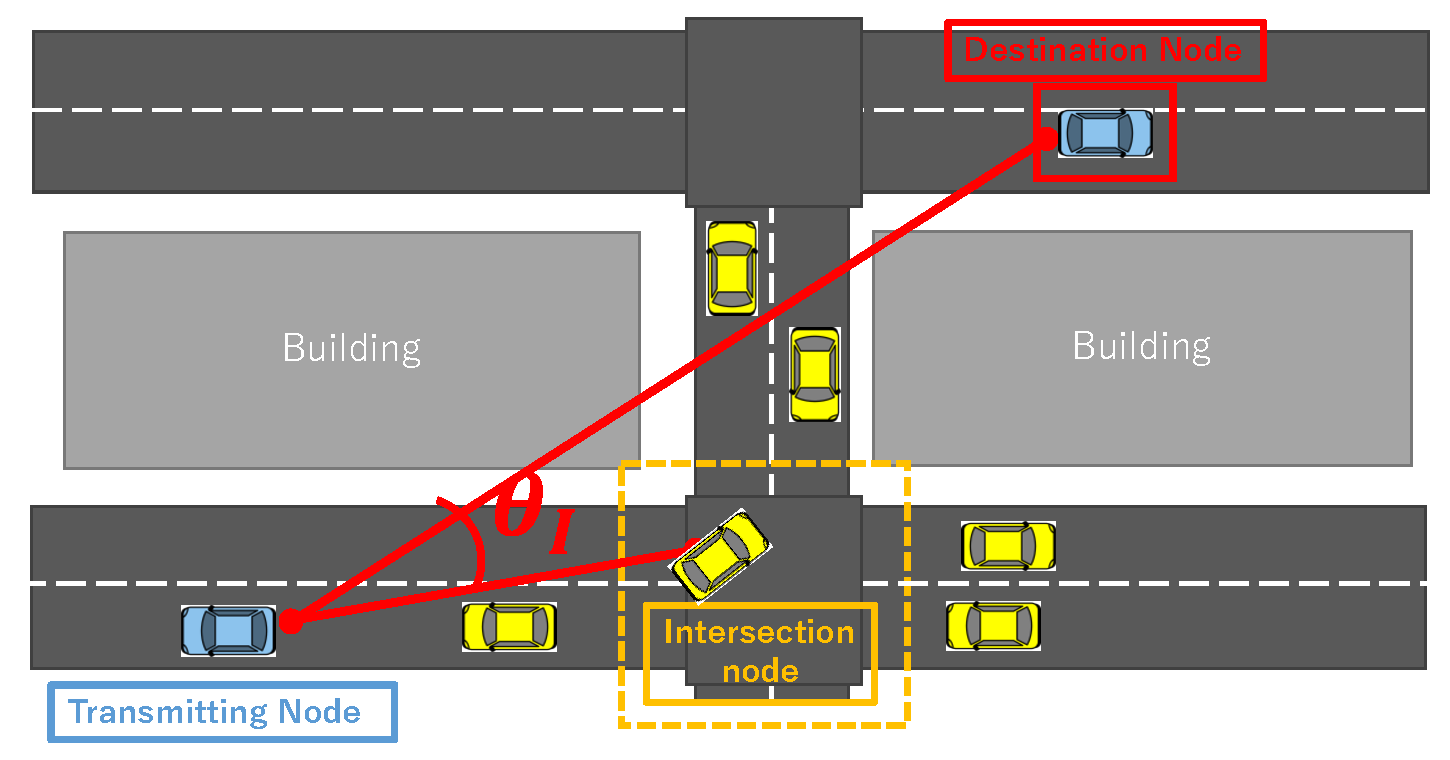
\includegraphics[width=90mm]{figures/Intersection_angle.eps}
\caption{The Intersection node angle}
\label{fig:intersection_angle}
\end{figure}


% \subsection{Neighbor status prediction algorithm}
% \label{neighbor_status}
% In most geographic routing protocols, each node obtains the location information of its neighboring nodes from the  information in the hello packets sent by neighboring nodes.
% However, the information in a hello packet may become outdated if the hello packet cannot be received or if the transmission interval is long.
% Therefore, in SIGO, the neighbor status prediction precisely identifies which roads or intersections neighboring vehicles exist. 
% The neighbor status prediction algorithm improves the accuracy of the priority calculation of street intersection nodes and can remove the broken link nodes from the relay candidate nodes. This algorithm can be divided into two steps:
% \subsubsection{Position prediction algorithm}

% The transmitting node predicts the position of its selected candidate  node based on the information in the candidate node's hello.
% packets. 
% The predicted neighbor node coordinates $x'$ and $y'$ are calculated using Equation \ref{position-prediction}.

% \begin{equation}
% \label{position-prediction}
% \begin{cases}
% x' = x + \left\{v(t-t_l) + \frac{1}{2}a(t-t_l)^2\right\}cos\theta, \\
% y' = y + \left\{v(t-t_l) + \frac{1}{2}a(t-t_l)^2\right\}sin\theta, \\
% \end{cases}
% \end{equation}

% In this equation, $a$, $v$, and $\theta$ are the information in the hello packet received by the transmitting node at time $t_l$ . where $t$ denotes the current time.

% \subsubsection{Prediction of broken links}
% The transmitting node estimates the distance between itself and its neighboring node using the predicted position information and predicts the broken link node before transmitting the data packet. The transmitting node removes neighbor node $i$ from the relay candidate nodes if the following condition is satisfied:


% \begin{equation}
% \label{expired_links}
% \sqrt{\left(x_s - x_i'\right)^2 + \left(y_s - y_i'\right)} > maxRange
% \end{equation}
% In this inequality, $x_s$ and  $y_s$ are the coordinates of the  transmitting node, and $x_i'$i and $y_i'$i are the coordinates of the neighbor node $i$.
% The left-hand side is the predicted distance between the transmitting node and the neighboring node at time $t$, and the right-hand side $maxRange$ is the threshold for detecting link breakage.


\subsection{Priority scheduling algorithm}
\label{priority}
In SIGO, a timer-based priority scheduling algorithm is used. 
In this algorithm, the node with the highest priority rebroadcasts the data packet first. 
When other relay candidate nodes overhear packets from nodes with a higher priority, they discard their pending packets. Each relay candidate node rebroadcasts the packet only when it has not received any packet from the node with a higher priority than itself until its timer expires.
In SIGO, the priority of node $i$ is calculated by the following equations (\ref{pri-intersection}) and (\ref{pri}).


\begin{equation}
\label{pri-intersection}
\frac{D_{sd} - D_{id}}{ETX_{i}^{2}} + IRI_i,  D_{id} < D_{sd}
\end{equation}

\begin{equation}
\label{pri}
\frac{D_{sd} - D_{id}}{ETX_{i}^{2}} ,   D_{id} < D_{sd}
\end{equation}

$D_{sd}$ is the distance from the transmitting node to the destination node, and $D_{id}$ is the distance from the relay candidate node $i$ to the destination node. If the condition $D_{id}$ < $D_{sd}$ is not satisfied, the node is excluded from the relay candidate nodes without calculating the priority. 
Equation (\ref{pri-intersection}) is applied when node $i$ is a street intersection node, and equation (\ref{pri}) is applied when node $i$ is located outside the intersection. 
The larger the value calculated by equation (\ref{pri-intersection}) or (\ref{pri}), the higher the priority is assigned to node $i$. 


\section{Performance evaluation}
\label{evaluation}
To evaluate the usefulness of the proposed protocol, we compared it with the LSGO protocol for three evaluation items: packet delivery ratio (PDR), end-to-end delay, and overhead.
The simulation parameters are shown in Table \ref{tab:parameter}. 
The simulation topology scenario was created using SUMO \cite{27}, as shown in Figure \ref{fig:scenario}. 

\begin{figure}[!ht]
\centering
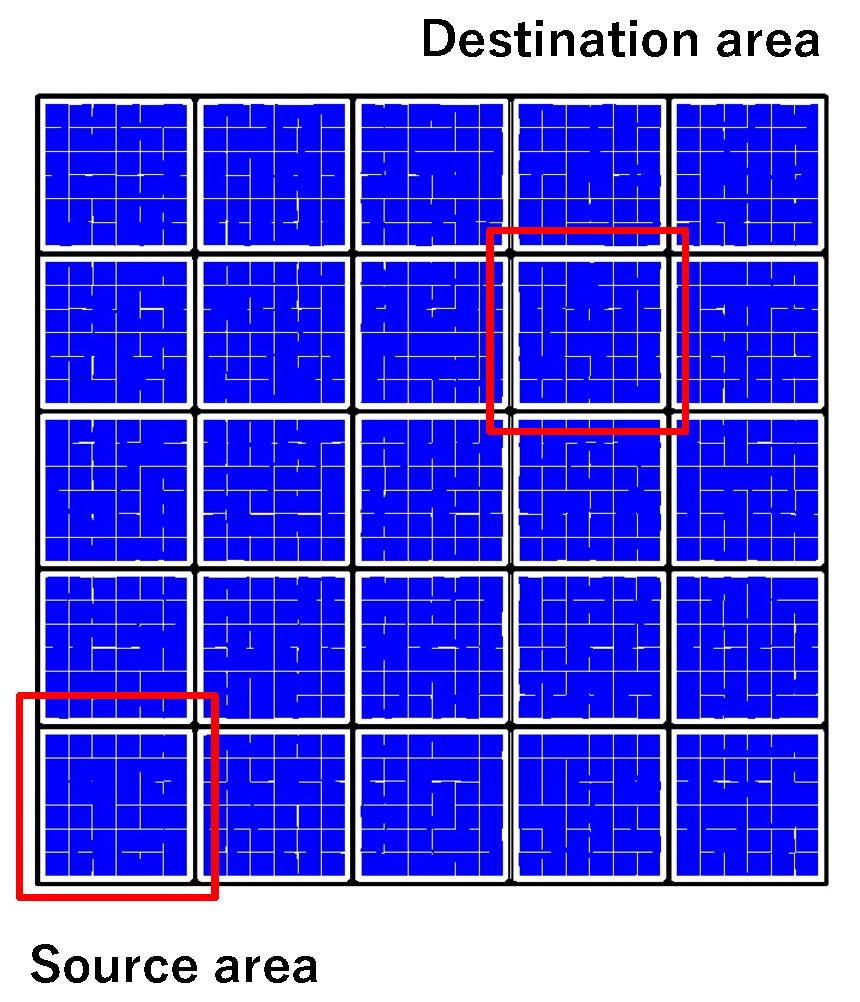
\includegraphics[width=50mm]{figures/scenario.eps}
\caption{simulation scenario }
\label{fig:scenario}
\end{figure}


Ten source node and destination node pairs were randomly selected from the source and destination areas in Figure \ref{fig:scenario}.
 Traffic signals were placed at each intersection, and buildings were placed as shown in the blue area of Figure \ref{fig:scenario}. 
The obstacle shadowing model \cite{20} was used as the radio wave propagation model. The obstacle shadowing propagation loss $L_{s,o}$ is calculated based on the loss for each wall and the distance (m) through the building, as shown in Equation (\ref{shadowing}).

\begin{equation}
\label{shadowing}
L_{s,o} = \alpha n  + \beta d_0
\end{equation}

where $\alpha$ is the attenuation per wall (dB), and $n$ is the number of walls penetrated. 
$\beta$ is the attenuation per meter (dB), and $d_0$ is the distance traveled through obstacles (m). 
In this simulation experiment, We evaluated the performance by varying the number of nodes and the shadowing parameter $\alpha$ in Equation (\ref{shadowing}). $\beta$ was fixed to 0.4db.  
An optimized algorithm to select the number of relay candidate nodes was proposed in LSGO. However, the performance of this algorithm is poor in the situations where shadowing occurs. For this reason, this evaluation fixed the maximum number of relay candidate nodes for both SIGO and LSGO.



\begin{table}[!ht]
\begin{center}
\caption{Simulation parameter}
\label{tab:parameter}
\begin{tabular}{|l|l|lll}
\cline{1-2}
Simulator    & NS-3 (v3.30) &  &  &  \\ \cline{1-2}
Simulation area    & 1000m × 1000m   &  &  &  \\ \cline{1-2}
Transmission range & 250m            &  &  &  \\ \cline{1-2}
Number of vehicles & 200, 300, 400      &  &  &  \\ \cline{1-2}
Radio propagation model    & obstacle shadowing model\cite{20}&  &  &  \\ \cline{1-2}
MAC Layer     & 802.11p &  &  &  \\ \cline{1-2}
Packet Size & 512 byte       &  &  &  \\ \cline{1-2}
Simulation Time & 30 s      &  &  &  \\ \cline{1-2}
hello interval & 1 s      &  &  &  \\ \cline{1-2}
Window size w  & 10 s      &  &  &  \\ \cline{1-2}
Number of relay candidate nodes  & 5       &  &  \\ \cline{1-2}
shadowing parameter $\alpha$  & 10db, 20db, 30db       &  &  &  \\ \cline{1-2}
shadowing parameter $\beta$    & 0.4db &  &  \\ \cline{1-2}
\end{tabular}
\end{center}
\end{table}





We evaluated the performance by varying the number of nodes and the shadowing parameter $\alpha$ in Equation \ref{shadowing}. 
$\beta$ was fixed to 0.4db.





Figure \ref{fig:PDR} shows the PDR of SIGO and LSGO when the number of nodes and the shadowing parameter is varied. 
In this figure, the number in round brackets after the protocol name indicates the value of the shadowing parameter $\alpha$. SIGO (10) shows the PDR of the proposed protocol when $\alpha$ is 10.
As shown in figure \ref{fig:PDR}, SIGO achieves a higher PDR than LSGO for all cases. 
As the number of nodes increased and the value of the shadowing parameter decreased, the PDR increased. This is because the possibility of forming an unreachable route (as shown in figure \ref{fig:LSGO-route}) increases in LSGO with an increase in $\alpha$. The possibility of forming a reachable route increases by prioritizing street intersection nodes in the SIGO.
We can also observe that the PDR of SIGO increases as the number of nodes increases compared to that of LSGO. It is assumed that this is due to an increase in the probability of the existence of nodes in the intersection. 
This  is because the probability of intersection nodes increases according to the number of nodes.

\begin{figure}[!ht]
\centering
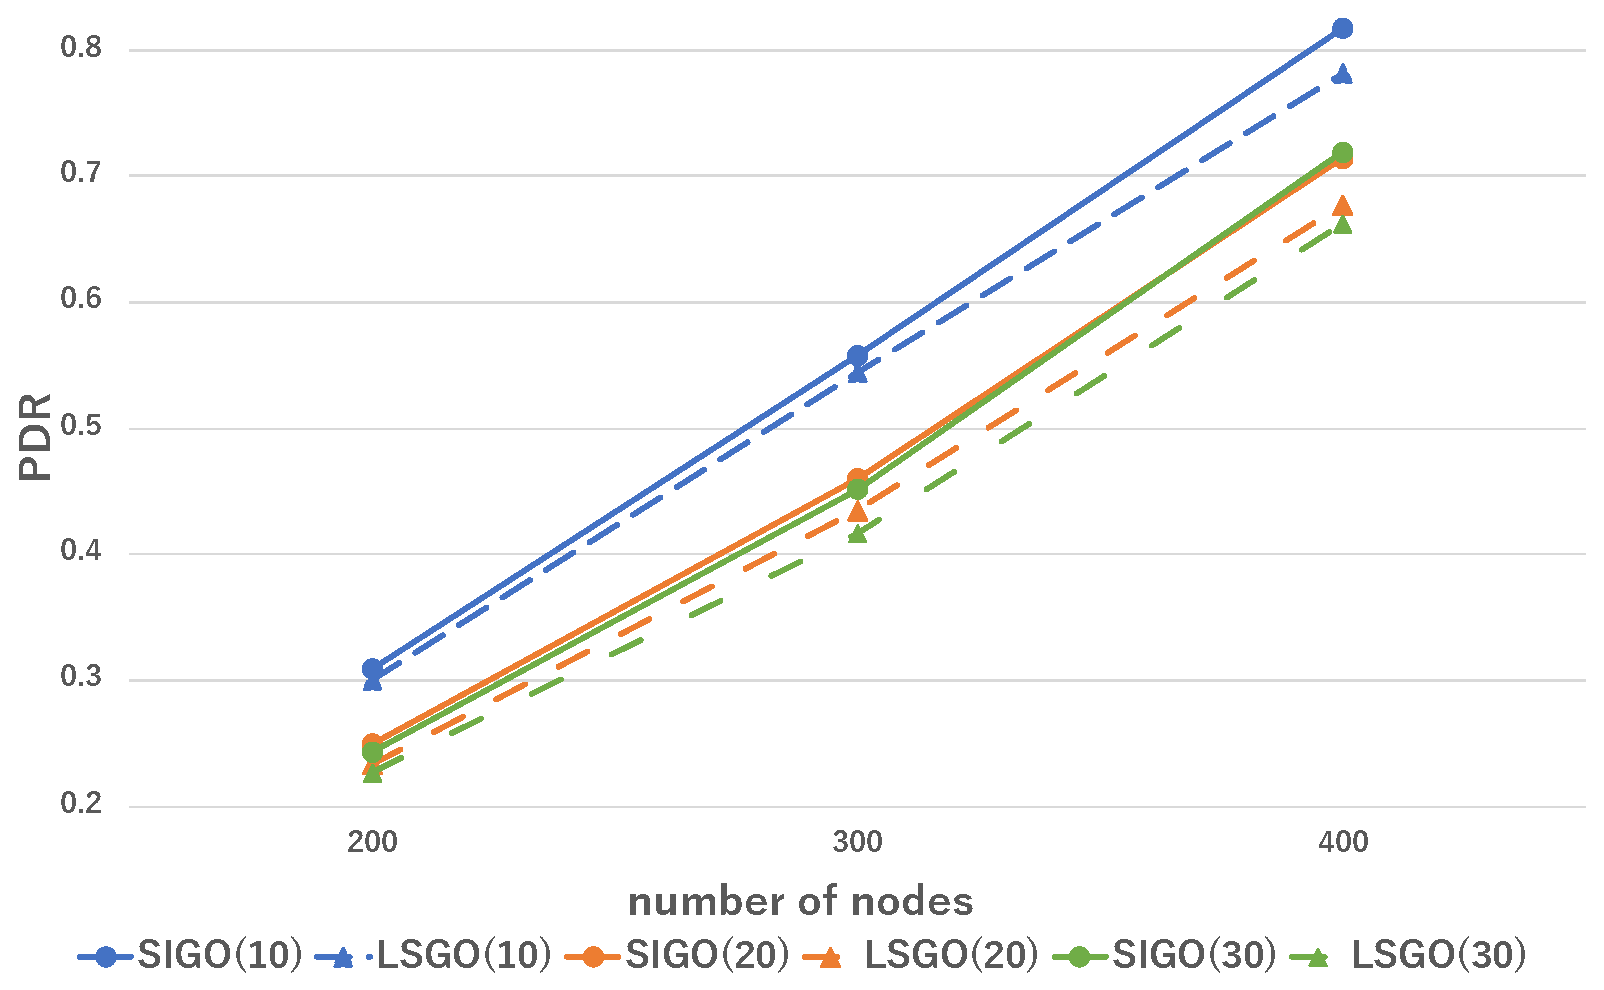
\includegraphics[width=80mm]{figures/PDR.eps}
\caption{Packet delivery ratio vs. number of nodes and shadowing intensity}
\label{fig:PDR}
\end{figure}


Figure \ref{fig:delay} shows the end-to-end delay of SIGO and LSGO when the number of nodes and the shadowing parameter are varied. 
As shown in figure \ref{fig:delay}, the delay of both SIGO and LSGO increases with an increase in the number of nodes. In the simulation scenario and setting of this study, the effect of the proposed protocol on the delay was very small. 
We have the following three reasons for this: 
(1) Because the road structure used in our simulation is a grid, the distance between the source node and the destination node does not change regardless of which road the packet is relayed on.
(2) In this experiment, we did not implement recovery routing such as the GPSR recovery scheme to deal with the local optimum problem. (3) Retransmission control was not used in the experiment.







\begin{figure}[!ht]
\centering
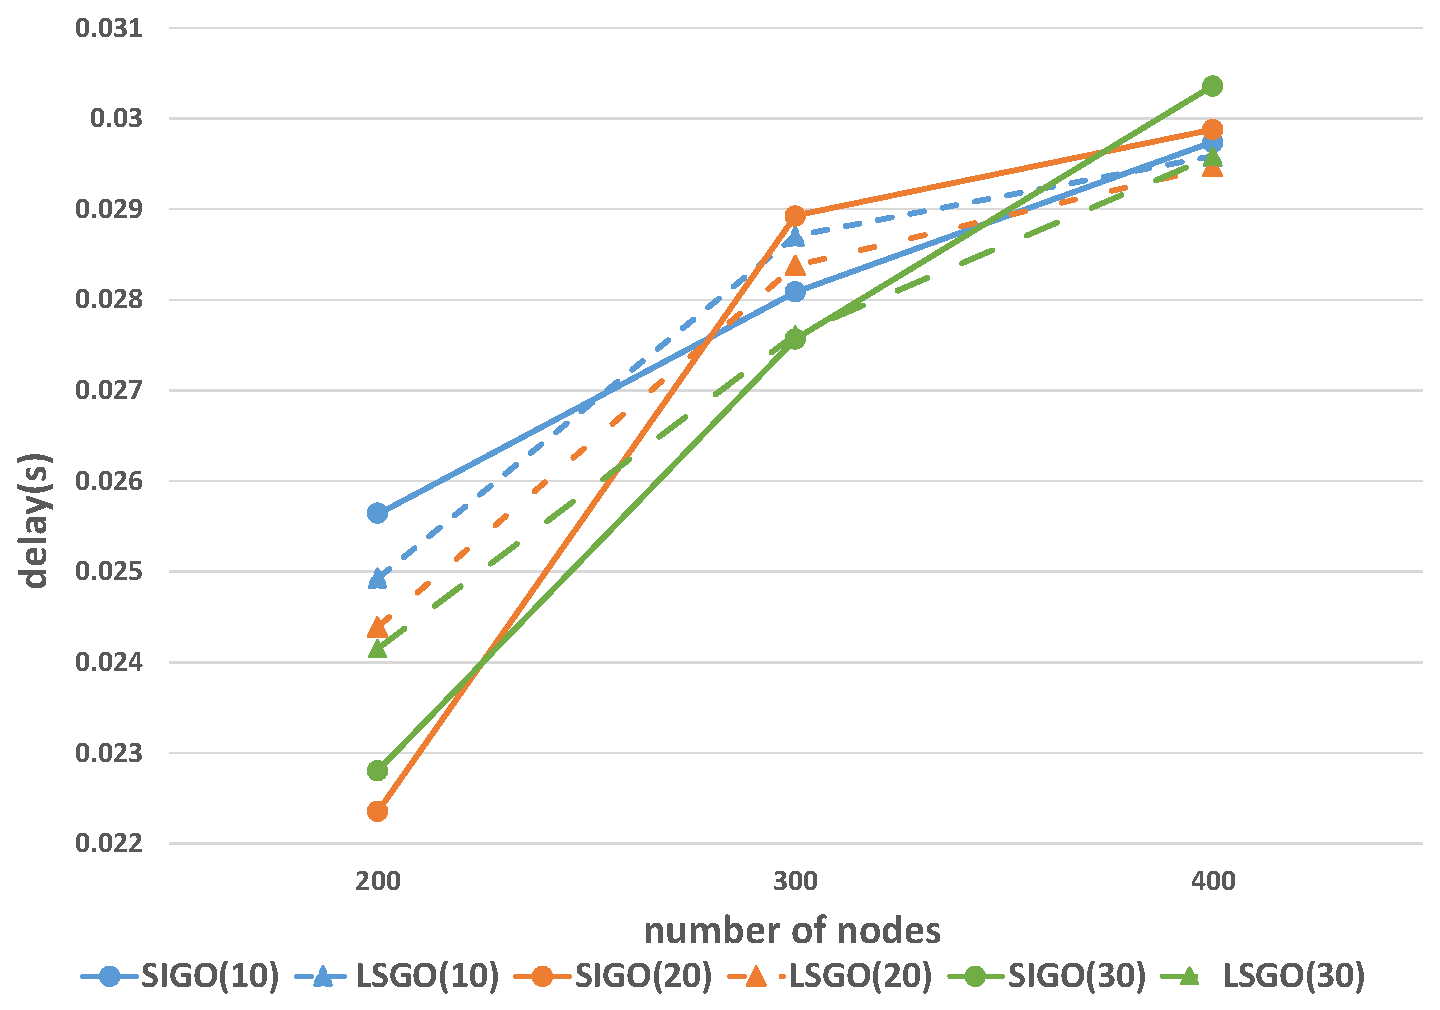
\includegraphics[width=80mm]{figures/delay.eps}
\caption{End-to-end delays vs. number of nodes and shadowing intensity }
\label{fig:delay}
\end{figure}



Figure \ref{fig:overhead} shows the overhead of SIGO and LSGO when the number of nodes and the shadowing parameter are varied. Figure 15 tells us: (1) The overhead of both LSGO and SIGO decreases with an increase in the number of nodes; (2) the overhead improvement of SIGO over LSGO increases with an increase in the shadowing parameter; (3) the difference in overhead between SIGO and LSGO becomes smaller with an increase in the number of nodes. The reason for (1) is that the total number of data packets successfully received by the destination node increases for both LSGO and SIGO, increasing the number of nodes. The reason for (2) is that the total number of data packets successfully received by the destination node increases in SIGO than in LSGO, increasing the shadowing parameter. In addition, this means that even though the total number of data packets successfully received by destination nodes increases in SIGO, the total number of data packets transmitted by all nodes does not increase significantly compared to LSGO. The reason for (3) is that when the number of nodes is large, rebroadcasting by the intersection node does not always result in efficient communication. Suppose there is a building in the direction of the destination node and a street intersection node rebroadcasts the packet in SIGO. In that case, nodes on two different roads forming the intersection are likely to be selected as relay candidate nodes when the number of nodes large. In this situation, the possibility that a low priority candidate node cannot receive packets from a high-priority relay candidate node due to the shadowing effect of a building increases. As a result, redundant rebroadcasting increases because the rebroadcasting by a low-priority relay candidate node is not canceled. Figure \ref{fig:overhead_reason} shows an example of this situation. The packets rebroadcasted by the street intersection node are received by nodes 1-4. Nodes 1, 2, 3, and 4 have a higher priority in that order. Ideally, only node 1 should rebroadcast the data packet. However, even if node 1 rebroadcasts the packet, nodes 3 and 4 cannot receive it due to the shadowing effect and rebroadcast.






\begin{figure}[!ht]
\centering
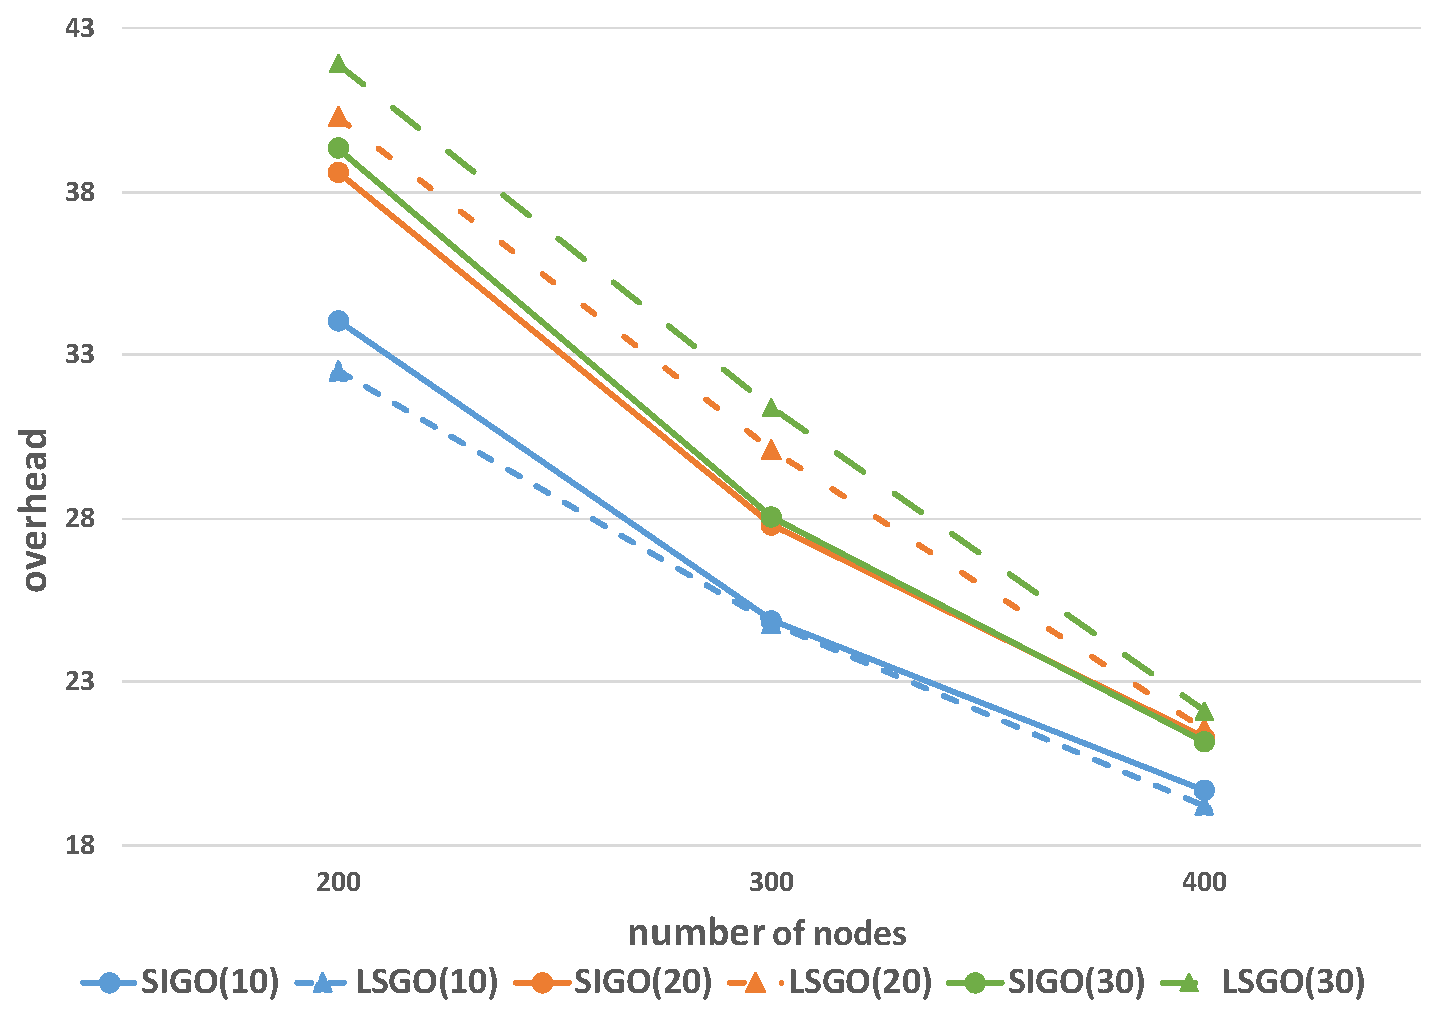
\includegraphics[width=90mm]{figures/overhead.eps}
\caption{Routing protocol overhead vs. number of nodes and shadowing intensity }
\label{fig:overhead}
\end{figure}

\begin{figure}[!ht]
\centering
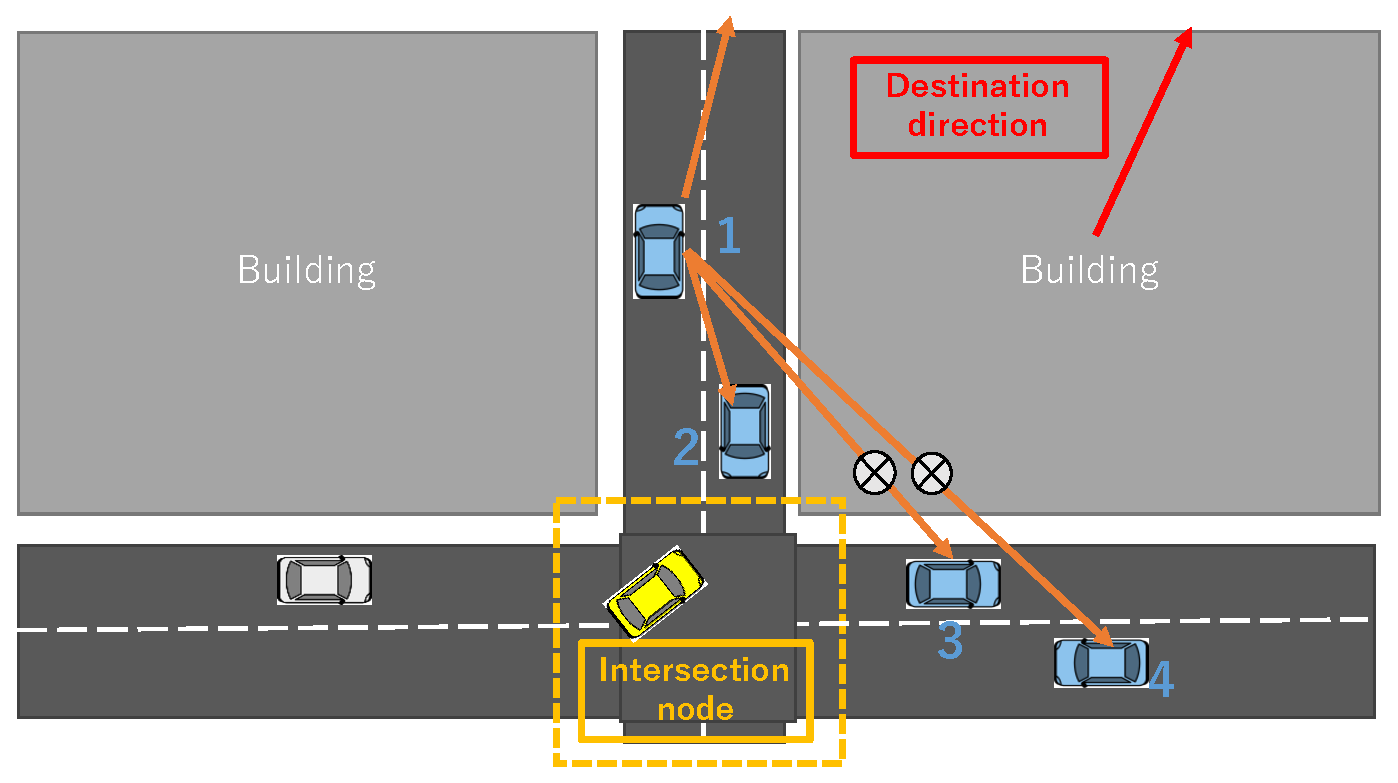
\includegraphics[width=85mm]{figures/overhead_reason.eps}
\caption{Causes of increased overhead}
\label{fig:overhead_reason}
\end{figure}



\section{Conclusion}
\label{conclusion}
We evaluated an existing opportunistic routing protocol under the impact of shadowing in a simulation. We demonstrated that the existing routing protocol degrades the communication performance when the effect of shadowing fading is considered in the simulation. 
We also proposed SIGO, which forms routes that are less susceptible to shadowing, and demonstrated its effectiveness in terms of improving the packet delivery ratio and reducing the overhead. 
Future work should include optimizing the number of relay candidate nodes, which was set to a fixed value in  our experiments. Furthermore, we plan to evaluate more complex simulation scenarios and redesign the SIGO routing protocol to support  various scenarios.


%\newpage

\bibliographystyle{IEEEtran}
\bibliography{shuto}


\begin{IEEEbiography}[{
\includegraphics[width=1in,height=1.25in,clip,keepaspectratio]{TakahashiShuto.eps}}]{Shuto Takahashi}
Received his B.E.degrees in Engineering from Ritsumeikan University in 2020. He enterd same university in April 2020, where he is currently master's student. His current research interests include vehicular ad-hoc networks.
\end{IEEEbiography}
% \vspace{-17cm}
\begin{IEEEbiography}[{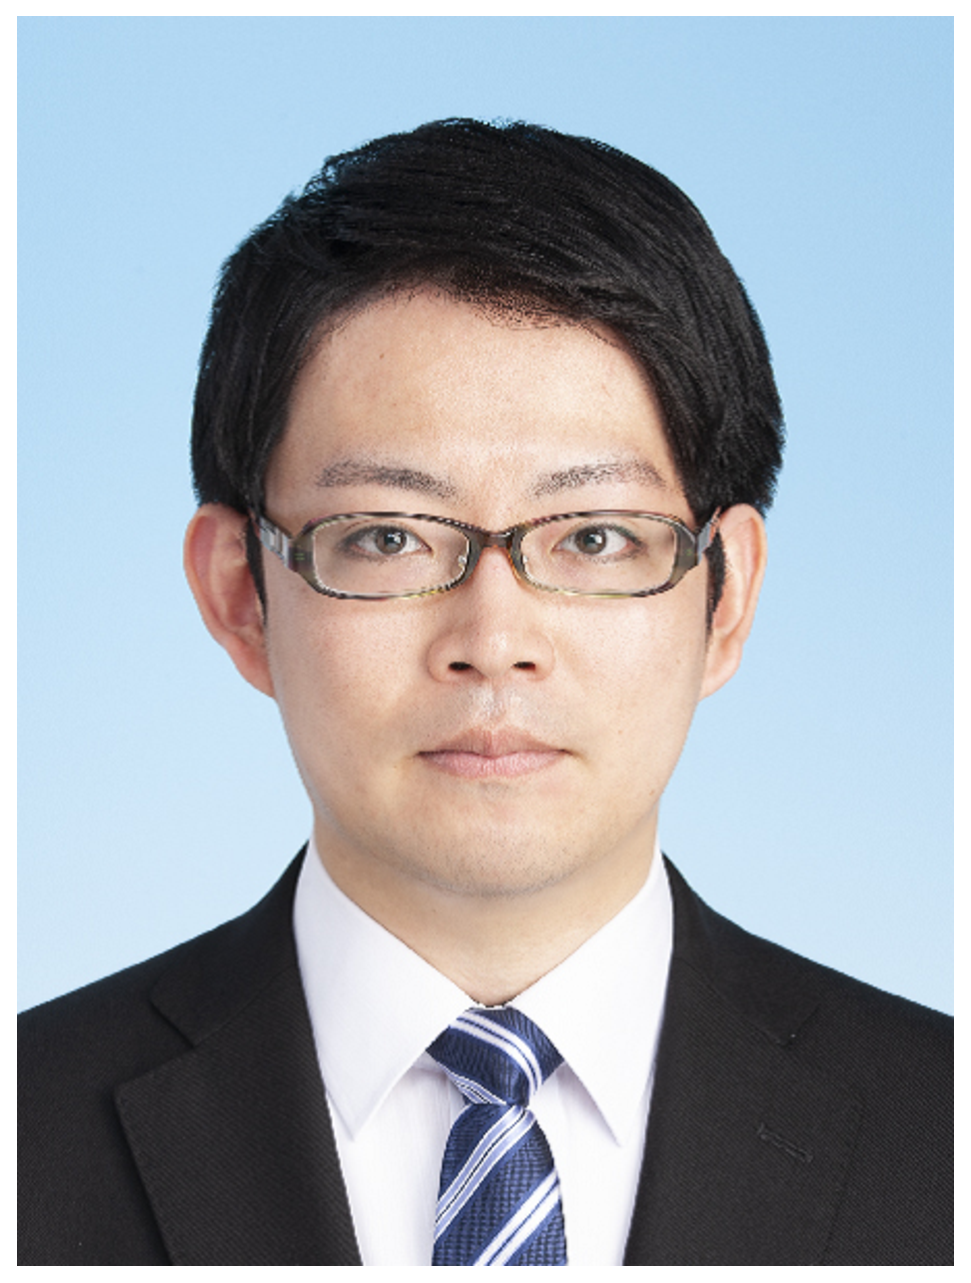
\includegraphics[width=1in,height=1.25in,clip,keepaspectratio]{YoshidaMasami.eps}}]{Masami Yoshida}
Received his B.E., M.E. degrees in Engineering from Ritsumeikan University in 2016 and 2018 respectively. He  enterd same university in April 2018, where he is currently Ph.d student. His current research interests include network coding, and ad-hoc networks.
\end{IEEEbiography}
\begin{IEEEbiography}[{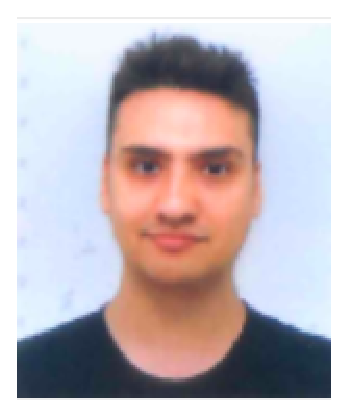
\includegraphics[width=1in,height=1.25in,clip,keepaspectratio]{Gallegos.eps}}]{Alberto Gallegos}
Received his M.S. and Ph.D. degrees in Engineering from Ritsumeikan University in 2014 and 2018 respectively. From April 2018 to September 2021, he was an Assistant Professor at the same University. He joined the Graduate School of Technology, Industrial and Social Sciences at Tokushima University in October 2021, where he is currently Assistant Professor. His current research interests include but are not limited to Wireless Sensor Networks, data mining, routing protocols, MAC layer designs and Internet of things applications.
\end{IEEEbiography}
\vspace{-17cm}
\begin{IEEEbiography}[{
\includegraphics[width=1in,height=1.25in,clip,keepaspectratio]{NoguchiTaku.eps}}]{Taku Noguchi}
He received the B.E., M.E., and Ph.D. degrees in communications 
engineering from Osaka University, Osaka, Japan in 2000, 2002, and 2004, 
respectively. He joined the College of Information Science and 
Engineering at Ritsumeikan University in 2004, where he is currently a 
professor. His research interests include performance analysis and the 
design of computer networks and wireless networks. He received the best 
tutorial paper award from IEICE ComSoc in 2012. He is a member of the 
IEEE, IEICE, and IPSJ.
\end{IEEEbiography}


\end{document}

